% Options for packages loaded elsewhere
\PassOptionsToPackage{unicode,}{hyperref}
\PassOptionsToPackage{hyphens}{url}
%
\documentclass[
  ]{scrartcl}
\usepackage{amsmath,amssymb}
\usepackage{iftex}
\ifPDFTeX
  \usepackage[T1]{fontenc}
  \usepackage[utf8]{inputenc}
  \usepackage{textcomp} % provide euro and other symbols
\else % if luatex or xetex
  \usepackage{unicode-math} % this also loads fontspec
  \defaultfontfeatures{Scale=MatchLowercase}
  \defaultfontfeatures[\rmfamily]{Ligatures=TeX,Scale=1}
\fi
\usepackage{lmodern}
\ifPDFTeX\else
  % xetex/luatex font selection
\fi
% Use upquote if available, for straight quotes in verbatim environments
\IfFileExists{upquote.sty}{\usepackage{upquote}}{}
\IfFileExists{microtype.sty}{% use microtype if available
  \usepackage[]{microtype}
  \UseMicrotypeSet[protrusion]{basicmath} % disable protrusion for tt fonts
}{}
\makeatletter
\@ifundefined{KOMAClassName}{% if non-KOMA class
  \IfFileExists{parskip.sty}{%
    \usepackage{parskip}
  }{% else
    \setlength{\parindent}{0pt}
    \setlength{\parskip}{6pt plus 2pt minus 1pt}}
}{% if KOMA class
  \KOMAoptions{parskip=half}}
\makeatother
\usepackage{xcolor}
\usepackage{color}
\usepackage{fancyvrb}
\newcommand{\VerbBar}{|}
\newcommand{\VERB}{\Verb[commandchars=\\\{\}]}
\DefineVerbatimEnvironment{Highlighting}{Verbatim}{commandchars=\\\{\}}
% Add ',fontsize=\small' for more characters per line
\newenvironment{Shaded}{}{}
\newcommand{\AlertTok}[1]{\textcolor[rgb]{1.00,0.00,0.00}{\textbf{#1}}}
\newcommand{\AnnotationTok}[1]{\textcolor[rgb]{0.38,0.63,0.69}{\textbf{\textit{#1}}}}
\newcommand{\AttributeTok}[1]{\textcolor[rgb]{0.49,0.56,0.16}{#1}}
\newcommand{\BaseNTok}[1]{\textcolor[rgb]{0.25,0.63,0.44}{#1}}
\newcommand{\BuiltInTok}[1]{\textcolor[rgb]{0.00,0.50,0.00}{#1}}
\newcommand{\CharTok}[1]{\textcolor[rgb]{0.25,0.44,0.63}{#1}}
\newcommand{\CommentTok}[1]{\textcolor[rgb]{0.38,0.63,0.69}{\textit{#1}}}
\newcommand{\CommentVarTok}[1]{\textcolor[rgb]{0.38,0.63,0.69}{\textbf{\textit{#1}}}}
\newcommand{\ConstantTok}[1]{\textcolor[rgb]{0.53,0.00,0.00}{#1}}
\newcommand{\ControlFlowTok}[1]{\textcolor[rgb]{0.00,0.44,0.13}{\textbf{#1}}}
\newcommand{\DataTypeTok}[1]{\textcolor[rgb]{0.56,0.13,0.00}{#1}}
\newcommand{\DecValTok}[1]{\textcolor[rgb]{0.25,0.63,0.44}{#1}}
\newcommand{\DocumentationTok}[1]{\textcolor[rgb]{0.73,0.13,0.13}{\textit{#1}}}
\newcommand{\ErrorTok}[1]{\textcolor[rgb]{1.00,0.00,0.00}{\textbf{#1}}}
\newcommand{\ExtensionTok}[1]{#1}
\newcommand{\FloatTok}[1]{\textcolor[rgb]{0.25,0.63,0.44}{#1}}
\newcommand{\FunctionTok}[1]{\textcolor[rgb]{0.02,0.16,0.49}{#1}}
\newcommand{\ImportTok}[1]{\textcolor[rgb]{0.00,0.50,0.00}{\textbf{#1}}}
\newcommand{\InformationTok}[1]{\textcolor[rgb]{0.38,0.63,0.69}{\textbf{\textit{#1}}}}
\newcommand{\KeywordTok}[1]{\textcolor[rgb]{0.00,0.44,0.13}{\textbf{#1}}}
\newcommand{\NormalTok}[1]{#1}
\newcommand{\OperatorTok}[1]{\textcolor[rgb]{0.40,0.40,0.40}{#1}}
\newcommand{\OtherTok}[1]{\textcolor[rgb]{0.00,0.44,0.13}{#1}}
\newcommand{\PreprocessorTok}[1]{\textcolor[rgb]{0.74,0.48,0.00}{#1}}
\newcommand{\RegionMarkerTok}[1]{#1}
\newcommand{\SpecialCharTok}[1]{\textcolor[rgb]{0.25,0.44,0.63}{#1}}
\newcommand{\SpecialStringTok}[1]{\textcolor[rgb]{0.73,0.40,0.53}{#1}}
\newcommand{\StringTok}[1]{\textcolor[rgb]{0.25,0.44,0.63}{#1}}
\newcommand{\VariableTok}[1]{\textcolor[rgb]{0.10,0.09,0.49}{#1}}
\newcommand{\VerbatimStringTok}[1]{\textcolor[rgb]{0.25,0.44,0.63}{#1}}
\newcommand{\WarningTok}[1]{\textcolor[rgb]{0.38,0.63,0.69}{\textbf{\textit{#1}}}}
\usepackage{longtable,booktabs,array}
\usepackage{calc} % for calculating minipage widths
% Correct order of tables after \paragraph or \subparagraph
\usepackage{etoolbox}
\makeatletter
\patchcmd\longtable{\par}{\if@noskipsec\mbox{}\fi\par}{}{}
\makeatother
% Allow footnotes in longtable head/foot
\IfFileExists{footnotehyper.sty}{\usepackage{footnotehyper}}{\usepackage{footnote}}
\makesavenoteenv{longtable}
\usepackage{graphicx}
\makeatletter
\def\maxwidth{\ifdim\Gin@nat@width>\linewidth\linewidth\else\Gin@nat@width\fi}
\def\maxheight{\ifdim\Gin@nat@height>\textheight\textheight\else\Gin@nat@height\fi}
\makeatother
% Scale images if necessary, so that they will not overflow the page
% margins by default, and it is still possible to overwrite the defaults
% using explicit options in \includegraphics[width, height, ...]{}
\setkeys{Gin}{width=\maxwidth,height=\maxheight,keepaspectratio}
% Set default figure placement to htbp
\makeatletter
\def\fps@figure{htbp}
\makeatother
\ifLuaTeX
  \usepackage{luacolor}
  \usepackage[soul]{lua-ul}
\else
  \usepackage{soul}
\fi
\setlength{\emergencystretch}{3em} % prevent overfull lines
\providecommand{\tightlist}{%
  \setlength{\itemsep}{0pt}\setlength{\parskip}{0pt}}
\setcounter{secnumdepth}{-\maxdimen} % remove section numbering
% definitions for citeproc citations
\NewDocumentCommand\citeproctext{}{}
\NewDocumentCommand\citeproc{mm}{%
  \begingroup\def\citeproctext{#2}\cite{#1}\endgroup}
\makeatletter
 % allow citations to break across lines
 \let\@cite@ofmt\@firstofone
 % avoid brackets around text for \cite:
 \def\@biblabel#1{}
 \def\@cite#1#2{{#1\if@tempswa , #2\fi}}
\makeatother
\newlength{\cslhangindent}
\setlength{\cslhangindent}{1.5em}
\newlength{\csllabelwidth}
\setlength{\csllabelwidth}{3em}
\newenvironment{CSLReferences}[2] % #1 hanging-indent, #2 entry-spacing
 {\begin{list}{}{%
  \setlength{\itemindent}{0pt}
  \setlength{\leftmargin}{0pt}
  \setlength{\parsep}{0pt}
  % turn on hanging indent if param 1 is 1
  \ifodd #1
   \setlength{\leftmargin}{\cslhangindent}
   \setlength{\itemindent}{-1\cslhangindent}
  \fi
  % set entry spacing
  \setlength{\itemsep}{#2\baselineskip}}}
 {\end{list}}
\usepackage{calc}
\newcommand{\CSLBlock}[1]{\hfill\break#1\hfill\break}
\newcommand{\CSLLeftMargin}[1]{\parbox[t]{\csllabelwidth}{\strut#1\strut}}
\newcommand{\CSLRightInline}[1]{\parbox[t]{\linewidth - \csllabelwidth}{\strut#1\strut}}
\newcommand{\CSLIndent}[1]{\hspace{\cslhangindent}#1}
\ifLuaTeX
\usepackage[bidi=basic]{babel}
\else
\usepackage[bidi=default]{babel}
\fi
\babelprovide[main,import]{american}
\babelprovide[import]{ngerman}
% get rid of language-specific shorthands (see #6817):
\let\LanguageShortHands\languageshorthands
\def\languageshorthands#1{}
\raggedbottom % or \flushbottom
% keep figures where there are in the text
\usepackage{float} 
\floatplacement{figure}{H}
% add custom hyphentation rules
\hyphenation
{%
  Hyphenate-me-like-this
  Dontyoueverhyphenateme
}%
\ifLuaTeX
  \usepackage{selnolig}  % disable illegal ligatures
\fi
\IfFileExists{bookmark.sty}{\usepackage{bookmark}}{\usepackage{hyperref}}
\IfFileExists{xurl.sty}{\usepackage{xurl}}{} % add URL line breaks if available
\urlstyle{same}
\hypersetup{
  pdftitle={Title},
  pdfauthor={Eleanor Roosevelt; John Peters Humphrey},
  pdflang={en-US},
  hidelinks,
  pdfcreator={LaTeX via pandoc}}

\title{Title\thanks{Many thanks for the valuable comments.}}
\usepackage{etoolbox}
\makeatletter
\providecommand{\subtitle}[1]{% add subtitle to \maketitle
  \apptocmd{\@title}{\par {\large #1 \par}}{}{}
}
\makeatother
\subtitle{Subtitle}
\author{\href{eleanor.eoosevelt@domain.com}{Eleanor
Roosevelt} \and \href{jph@domain.com}{John Peters Humphrey}}
\date{1 January 2023}

\begin{document}
\maketitle
\begin{abstract}
All human beings are born free and equal in dignity and rights. All
human beings are born free and equal in dignity and rights. All human
beings are born free and equal in dignity and rights. All human beings
are born free and equal in dignity and rights.
\end{abstract}



\renewcommand*\contentsname{Contents}
{
\setcounter{tocdepth}{2}
\tableofcontents
}
\listoffigures
\listoftables
\section{Heading 1}\label{heading-1}

All human beings are born free and equal in dignity and rights. All
human beings are born free and equal in dignity and rights. All human
beings are born free and equal in dignity and rights. All human beings
are born free and equal in dignity and rights.

\subsection{Heading 2}\label{heading-2}

All human beings are born free and equal in dignity and rights. All
human beings are born free and equal in dignity and rights. All human
beings are born free and equal in dignity and rights. All human beings
are born free and equal in dignity and rights.

\subsubsection{Heading 3}\label{heading-3}

All human beings are born free and equal in dignity and rights. All
human beings are born free and equal in dignity and rights. All human
beings are born free and equal in dignity and rights. All human beings
are born free and equal in dignity and rights.

\paragraph{Heading 4}\label{heading-4}

All human beings are born free and equal in dignity and rights. All
human beings are born free and equal in dignity and rights. All human
beings are born free and equal in dignity and rights. All human beings
are born free and equal in dignity and rights.

\subsection{Bold}\label{bold}

\textbf{All human beings are born free and equal in dignity and rights.}
All human beings are born free and equal in dignity and rights.All human
beings are born free and equal in dignity and rights.All human beings
are born free and equal in dignity and rights.

\subsection{Italic}\label{italic}

\emph{All human beings are born free and equal in dignity and rights.}
All human beings are born free and equal in dignity and rights.All human
beings are born free and equal in dignity and rights.All human beings
are born free and equal in dignity and rights.

\subsection{Bold and italic}\label{bold-and-italic}

\textbf{\emph{All human beings are born free and equal in dignity and
rights.}} All human beings are born free and equal in dignity and
rights.All human beings are born free and equal in dignity and
rights.All human beings are born free and equal in dignity and rights.

\subsection{Struck through}\label{struck-through}

\st{All human beings are born free and equal in dignity and rights.} All
human beings are born free and equal in dignity and rights.All human
beings are born free and equal in dignity and rights.All human beings
are born free and equal in dignity and rights.

\subsection{Numbered lists}\label{numbered-lists}

\begin{enumerate}
\def\labelenumi{\arabic{enumi}.}
\tightlist
\item
  All human beings are born free and equal in dignity and rights.
\item
  All human beings are born free and equal in dignity and rights.
\item
  All human beings are born free and equal in dignity and rights.
\item
  All human beings are born free and equal in dignity and rights.
\end{enumerate}

All human beings are born free and equal in dignity and rights. All
human beings are born free and equal in dignity and rights. All human
beings are born free and equal in dignity and rights. All human beings
are born free and equal in dignity and rights.

\subsection{Unnumbered lists}\label{unnumbered-lists}

\begin{itemize}
\tightlist
\item
  All human beings are born free and equal in dignity and rights.

  \begin{itemize}
  \tightlist
  \item
    All human beings are born free and equal in dignity and rights.
  \end{itemize}
\item
  All human beings are born free and equal in dignity and rights.
\end{itemize}

All human beings are born free and equal in dignity and rights. All
human beings are born free and equal in dignity and rights. All human
beings are born free and equal in dignity and rights. All human beings
are born free and equal in dignity and rights.

\subsection{Mixed lists}\label{mixed-lists}

\begin{itemize}
\tightlist
\item
  All human beings are born free and equal in dignity and rights.

  \begin{enumerate}
  \def\labelenumi{\arabic{enumi}.}
  \tightlist
  \item
    All human beings are born free and equal in dignity and rights.
  \item
    All human beings are born free and equal in dignity and rights.
  \end{enumerate}
\item
  All human beings are born free and equal in dignity and rights.
\end{itemize}

All human beings are born free and equal in dignity and rights. All
human beings are born free and equal in dignity and rights. All human
beings are born free and equal in dignity and rights. All human beings
are born free and equal in dignity and rights.

\subsection{Figures and captions}\label{figures-and-captions}

\begin{figure}
\centering
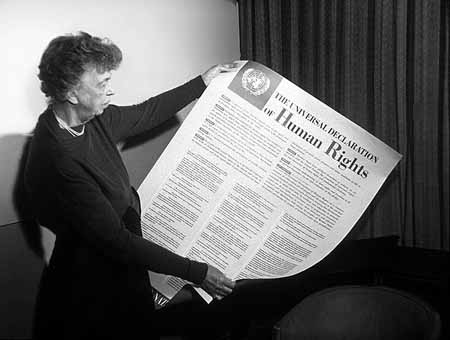
\includegraphics{images/Eleanor_Roosevelt_and_Human_Rights_Declaration.jpeg}
\caption{Eleanor Roosevelt hält die englische Version der Allgemeinen
Erklärung der Menschenrechte (FDR Presidential Library \& Museum, CC BY
2.0 \url{https://creativecommons.org/licenses/by/2.0}, via Wikimedia
Commons)}
\end{figure}

All human beings are born free and equal in dignity and rights. All
human beings are born free and equal in dignity and rights. All human
beings are born free and equal in dignity and rights. All human beings
are born free and equal in dignity and rights.

\subsection{Code}\label{code}

All human beings are born free and equal in dignity and rights. All
human beings are born free and equal in dignity and rights. All human
beings are born free and equal in dignity and rights. All human beings
are born free and equal in dignity and rights.

\begin{Shaded}
\begin{Highlighting}[]
\FunctionTok{ping}\NormalTok{ wikipedia.org}
\end{Highlighting}
\end{Shaded}

All human beings are born free and equal in dignity and rights. All
human beings are born free and equal in dignity and rights. All human
beings are born free and equal in dignity and rights. All human beings
are born free and equal in dignity and rights.

\subsection{URLs and email addresses}\label{urls-and-email-addresses}

\href{https://www.wikipedia.org/}{wikipedia.org},
\href{mailto:info@wikipedia.org}{\nolinkurl{info@wikipedia.org}}. All
human beings are born free and equal in dignity and rights. All human
beings are born free and equal in dignity and rights. All human beings
are born free and equal in dignity and rights. All human beings are born
free and equal in dignity and rights.

\subsection{Tables}\label{tables}

\begin{longtable}[]{@{}
  >{\raggedright\arraybackslash}p{(\columnwidth - 2\tabcolsep) * \real{0.5000}}
  >{\raggedright\arraybackslash}p{(\columnwidth - 2\tabcolsep) * \real{0.5000}}@{}}
\caption{Table caption}\tabularnewline
\toprule\noalign{}
\begin{minipage}[b]{\linewidth}\raggedright
column 1
\end{minipage} & \begin{minipage}[b]{\linewidth}\raggedright
column 2
\end{minipage} \\
\midrule\noalign{}
\endfirsthead
\toprule\noalign{}
\begin{minipage}[b]{\linewidth}\raggedright
column 1
\end{minipage} & \begin{minipage}[b]{\linewidth}\raggedright
column 2
\end{minipage} \\
\midrule\noalign{}
\endhead
\bottomrule\noalign{}
\endlastfoot
All human beings are born free and equal in dignity and rights. & All
human beings are born free and equal in dignity and rights. \\
All human beings are born free and equal in dignity and rights. & All
human beings are born free and equal in dignity and rights. \\
All human beings are born free and equal in dignity and rights. & All
human beings are born free and equal in dignity and rights. \\
All human beings are born free and equal in dignity and rights. & All
human beings are born free and equal in dignity and rights. \\
\end{longtable}

All human beings are born free and equal in dignity and rights. All
human beings are born free and equal in dignity and rights. All human
beings are born free and equal in dignity and rights. All human beings
are born free and equal in dignity and rights.

\subsection{Footnotes}\label{footnotes}

All human beings are born free and equal in dignity and rights. All
human beings are born free and equal in dignity and rights. All human
beings are born free and equal in dignity and rights. All human beings
are born free and equal in dignity and rights.\footnote{All human beings
  are born free and equal in dignity and rights.}

\subsection{Quotes}\label{quotes}

\begin{otherlanguage}{ngerman}

\begin{quote}
Alle Menschen sind frei und gleich an Würde und Rechten geboren.
\end{quote}

\end{otherlanguage}

All human beings are born free and equal in dignity and rights. All
human beings are born free and equal in dignity and rights. All human
beings are born free and equal in dignity and rights. All human beings
are born free and equal in dignity and rights.

\subsection{Scientific citations}\label{scientific-citations}

\begin{quote}
All human beings are born free and equal in dignity and rights. They are
endowed with reason and conscience and should act towards one another in
a spirit of brotherhood. United Nations\footnote{\emph{Universal
  Declaration of Human Rights}.}
\end{quote}

All human beings are born free and equal in dignity and rights. All
human beings are born free and equal in dignity and rights. All human
beings are born free and equal in dignity and rights. All human beings
are born free and equal in dignity and rights.\footnote{United Nations,
  \emph{Universal Declaration of Human Rights}.}

\section{Bibliography}\label{bibliography}

\phantomsection\label{refs}
\begin{CSLReferences}{1}{1}
\bibitem[\citeproctext]{ref-brown2016}
Brown, Gordon, ed. \emph{The {Universal} {Declaration} of {Human}
{Rights} in the 21st Century, a Living Document in a Changing World}.
Open Book Publishers ; NYU Global Institute for Advanced Study, 2016.

\bibitem[\citeproctext]{ref-unitednations1948}
United Nations. \emph{Universal Declaration of Human Rights}. 1948.

\end{CSLReferences}



\end{document}
